\documentclass[a4paper]{article}
\usepackage{geometry}
 \geometry{
 a4paper,
 total={210mm,297mm},
 left=1.25in,
 right=1.25in,
 top=1.25in,
 bottom=1.25in,
 }
\usepackage{graphicx}
%\usepackage[T1]{fontenc}
%\usepackage{todonotes}
%\usepackage{graphicx}
\usepackage{amsmath}
\usepackage{amssymb}
\usepackage{bbm}
\usepackage{tgpagella}
%\providecommand\refname{References}
\usepackage{graphicx}
\graphicspath{ {images/} }

\title{Portfolio Optimization with linear and fixed transaction costs}
\author{Ashok Vardhan \\ Sasank Chilamkurthy}


\begin{document}
\maketitle


\section{Introduction}

In this paper, we consider the problem of optimal portfolio selection, with transaction costs and constraints on exposure to risk, short-sell constraints, etc. Under the assumption of linear transaction costs (which might not be completely realistic ), bounds on the variance of the return, bounds on  different shortfall probabilities, the optimization problem of maximizing the asset-wealth is convex which can be solved efficiently.\\[0.2em]

Portfolio optimization problems with transaction costs that include a fixed fee, or discount
breakpoints, which are more realistic cannot be directly solved by convex optimization. We address this issue of non-convexity by solving a small number of related convex optimization problems which can be used to provide better bounds for the original optimization problem. Thus, this method only produces a sub-optimal solution with an upper bound on the original optimum. This method involves employing a heuristic which only yields a sub-optimal solution. However, the numerical results for several practical scenarios indicate that the gap between them is quite small.

The next section deals with the problem description in detail.

\section{Problem description}

\subsection{Objective function}

We consider an investment portfolio that consists of holdings in some or all of $n$ assets. Transactions performed on these assets adjust the portfolios which are then held for a fixed period of time. The goal of the investor is the maximize the expected wealth at the end of the period, such that the portfolios held satisfy  a set of constraints described below.\\[0.2em]

The current holds in the assets are given by the vector $w= [w_1,w_2,\ldots, w_n]^T$. The vector $x=[x_1,x_2,\ldots, x_n]^T$  denotes the transactions in each of these assets, with $x_i>0$ for buying and $x_i<0$ for selling. Thus the adjusted portfolio is given by $w+x$. \\

The portfolio $w+x$ is held for a fixed period of time. Return on each of the assets by the end of this period is given by a random variable (random vector) $a=[a_1,a_2,\ldots, a_n]^T$. We assume that mean and variance of $a$ are known.
$$
\mathbb{E}(a)= \bar{a},\ \mathbb{E} (a-\bar{a})^T (a-\bar{a}) =\Sigma
$$

The end of period wealth is a random variable, $W = a^T(w + x)$, with expected value and
variance given by
$$
\mathbb{E}(W) = \bar{a}^T(w+x), \ \mathbb{E}(W-\mathbb{E}(W))^2= (w+x)^T \Sigma (w+x).
$$

\subsection{Constraints}
\subsubsection{Self-financing constraint}

Let $\phi(x)$ denote the total transaction costs for the transactions $x$ described above. We assume the portfolio is self-financing, i.e there is no exogenous infusion or withdrawal of money; the purchase of a new asset must be financed by the sale of an old one.\cite{1} Mathematically,
$$
\mathbbm{1}^Tx + \phi(x) =0
$$

We consider a inequality version of the above which is more appropriate (for example, if $\phi$ is convex) and justified (both of them yielding same results) in \cite{2},
\begin{equation}
\mathbbm{1}^Tx + \phi(x)  \leq 0 
\end{equation}

Another motivation for considering (2) rather than (1) is that the latter needn't be convex.


We will describe the transaction costs in detail towards the end of this section with several variants.

\subsubsection{Shortselling constraints}

Shortselling constraints alead to linear inequalities. We impose 
individual bounds $s_i$ on the maximum amount of shortselling permissible on asset $i$, i.e,
\begin{equation}
w_i + x_i \geq -s_i, \ i = 1,\ldots, n.
\end{equation}

We can also handle other variants which are of more practical interest such as collaterization requirement along similar lines.\cite{2}

\subsubsection{Constraints on variance of wealth}

The standard deviation of the end of period wealth $W$ is constrained to be less than $\sigma_{max}$ by
the (convex) quadratic inequality
$$
(w + x)^T \Sigma (w + x) \leq \sigma_{max}^2,
$$
Equivalently,
\begin{equation}
\|\Sigma^{1/2}(w+x)\| \leq \sigma_{max}
\end{equation}

We define the returns on the initial wealth $\mathbbm{1}^Tw$ as $R =\frac{\bar{a}^T(w+x)}{\mathbbm{1}^Tw}$


The constraint (3) is a second-order conic constraint.
\subsubsection{Shortfall risk constraints}

We assume that the random vector for returns is Guassian, i.e $a \thicksim \mathcal{N}(\bar{a},\Sigma)$. We impose that the end-period wealth $W$ be greater than some undesired level $W^{low}$
with a confidence level $\eta$ (where $\eta \geq 0.5$), 
\[
\text{Prob}(W \geq W^{low}) \geq \eta
\]

Since we know that $W = a^T(w+x),$ we have $W \thicksim \mathcal{N}(\mu,\sigma^2)$, which implies
\begin{align*}
\text{Prob}(\frac{W-\mu}{\sigma} \leq \frac{W^{low}-\mu}{\sigma}) &\leq 1- \eta, & \\
 \Rightarrow \frac{W^{low}-\mu}{\sigma} &\leq \Phi^{-1}(1-\eta),&\\
\end{align*}

where $\Phi(z)$ is the cumulative distributive function for standard guassian.\\[0.2em]
Using the fact that $\Phi^{-1}(1-\eta)= \Phi^{-1}(\eta)$ and $\mu= \bar{a}^T(w+x),\ \sigma=\|\Sigma^{1/2}(w+x) \|$,

\begin{equation}
\Phi^{-1}(\eta)\|\Sigma^{1/2}(w+x)\| \leq \bar{a}^T(w+x)- W^{low}
\end{equation}

For $\eta \geq 0.5,\ \Phi^{-1}(\eta) \geq 0,$ and thus (4) is a convex quadratic constraint.\\

For the above shortfall constraint setting, we can also impose constraint on a merely
bad return, with some modest confidence, as well as a constraint on a truly disastrous return,
with much greater confidence.

\subsubsection{Transaction costs}

We assume that transaction cost is separable, i.e
$$
\phi(x) =\sum_{i=1}^n \phi_i(x_i)
$$
where $\phi_i$ is the transaction cost associated with trading asset $i$.

The two realistic variants of transaction costs that consider are linear transaction costs and fixed transaction costs. First consider the linear case:
\[
 \phi_i(x_i) =
  \begin{cases}
   \alpha_i^{+}x_i^+ & \text{if } x \geq 0 \\
   \alpha_i^{-}x_i^-       & \text{if } x \leq 0
  \end{cases}
\]

where $x_i = x_i^+ - x_i ^-,\ x_i^+ = \max\{x_i,0 \},\ x_i^- = \max\{-x_i,0\}$. Here $\alpha_i^+, \alpha_i^- \geq 0$ are the cost rates associated with buying and selling asset $i$. More succinctly, 
$$
\phi_i(x_i)= \alpha_i^{+}x_i^+ + \alpha_i^{-}x_i^-.
$$  

However in practice, transaction costs are not convex functions of the amount traded. Indeed, the
costs for either buying or selling are likely to be concave\cite{2}.\\
 We will consider a simple model that includes fixed
plus linear costs. Let $\beta_i^+$ and $\beta_i^-$ are the costs associated with selling and buying the asset $i$ respectively. Then the fixed-plus-linear transaction cost function is given by:
\[
 \phi_i(x_i) =
  \begin{cases}
   \beta_i^+ + \alpha_i^{+}x_i^+ &:  x > 0 \\
   \beta_i^- + \alpha_i^{-}x_i^-       &: x < 0\\
   0 &: x=0
  \end{cases}
\]

Clearly, $\phi_i(x_i)$ is not a convex function and poses a problem to the convexity of the optimization problem.

\begin{figure}[h]
\centering
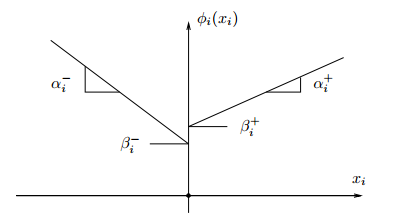
\includegraphics[width=8cm]{img.png}

\end{figure}
\newpage

\section{Optimization problem}
We pose the optimization problem of maximizing the wealth $W=a^T(w+x)$ subject to the constraints discussed above.

\subsection{Linear transaction costs}
We consider the transaction costs to be linear in this case. The corresponding optimization problem with short-fall risk constraints, short-selling constraints, self-financing constraint being included is given by:


\begin{equation}
\begin{aligned}
& \underset{x}{\text{maximize}}
& & \bar{a}^T (w+x^+ - x^-) \\
& \text{subject to}
& & \mathbbm{1}^Tx + \displaystyle \sum_{i=1}^n (\alpha_i^{+}x_i^+ + \alpha_i^{-}x_i^-) \leq 0  \\
& & & w_i +x_i^+ - x_i^-   \leq  s_i,  i=1,2,\ldots,n.\\
& & & \Phi^{-1}(\eta_j)\|\Sigma^{1/2}(w+x)\| \leq \bar{a}^T(w+x)- W_j^{low}, \  j=1,2 \\
& & &   x_i^+ \geq 0,\ x_i^- \geq 0,\ i=1,2,\ldots,n   \\
\end{aligned}
\end{equation}

It is obvious that (5) is a convex optimization problem since each of the constraints as well as objective function are convex.


\subsection{Fixed transaction costs}

The general transaction cost function is given by:
$$
\phi(x)= \sum_{i=1}^n \phi_i(x_i)
$$
with
\textsc{\[
 \phi_i(x_i) =
  \begin{cases}
   \beta_i + \alpha_i |x_i| & :  x > 0 \\
    0 &: x=0
  \end{cases}
\]
}
Costs such as above lead to a hard combinatorial optimization problem.\\

If the $\beta_i$ are very small, this may lead to an acceptable approximation. In general, however, it will generate inefficient solutions with too many transactions.\cite{2}

On the other hand, by considering the fixed costs, we discourage trading small amounts
of a large number of assets. Thus, we obtain a sparse vector of trades; i.e., one that has many
zero entries. This means most of the trading will be concentrated in a few assets, which is a
desirable property.\\[0.2em]

We will consider a heuristic for this fixed transaction costs case where the problem is non-convex. This procedure though yields only a sub-optimal solution, it is found to be quite good in practice with respect to the actual solution.

\subsubsection{Convex relaxation}

We assume that lower and upper bounds on the xi are known, i.e., $-l_i$ and $u_i$ for which $x_i$ must
satisfy:
$$
-l_i \leq x_i \leq u_i
$$
The convex
envelope of $\phi_i$ , which is the largest convex function which is lower or equal to $\phi_i$ in the interval
$[−l_i, u_i ],$ is given by:

\[
 \phi_i^{c.e}(x_i) =
  \begin{cases}
   \big(\frac{\beta_i}{u_i} + \alpha_i \big) x_i & :  x_i \geq  0 \\
    - \big(\frac{\beta_i}{l_i} + \alpha_i \big) x_i & :  x_i \leq 0 \\
  \end{cases}
\]
\begin{figure}[h]
\centering
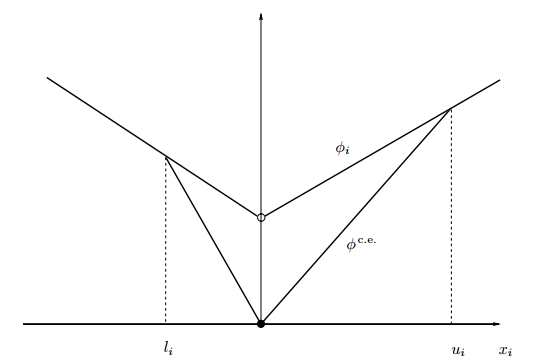
\includegraphics{convex.png}

\end{figure}

Since $\phi_i^{c.e}$ lower bounds $\phi_i$ , it enlarges the feasible set. Thus the optimal value for the convex relaxation problem is a upper  bound for the optimization problem. Thus we formulate the relaxed optimization problem:

\begin{equation}
\begin{aligned}
& \underset{x}{\text{maximize}}
& & \bar{a}^T (w+x^+ - x^-) \\
& \text{subject to}
& & \mathbbm{1}^Tx + \displaystyle \sum_{i=1}^n \phi_i^{c.e}(x_i) \leq 0  \\
& & & w+x \in \mathcal{S}\\
\end{aligned}
\end{equation}

where $\mathcal{S}$ refers to the set of feasible vectors $w+x$ similar to that of (5).\\

Since the problem (5) is convex, we can compute its optimal solution, and hence the upper
bound on the optimal value of the original problem (4), very efficiently.\\

If the optimal solution for the convex problem (5) is also a feasible solution for (4), it serves as the optimum for (4) as well. However, as we notice, $\phi_i$ and $\phi_i^{c.e}$ agree only on $0, u_i, -l_i$ and in practice, it is quite seldom.\\

The idea behind this convex relaxation is to replace the indicator function of a bounded variable with its convex envelope. This technique is refereed to as $\l_1$ norm relaxation.\cite{2}
\subsection{Heuristic algorithm}

Consider the following  procedure used to obtain the sub-optimal portfolio management.

\begin{enumerate}
\item
$k:=0.$\\
Solve the convex relaxed problem (5).\\
Let $x^0$ be the solution to the problem.\\
\item
$k=k+1$.\\
Given the solution to the previous problem $x^{k-1}$ , define $\hat{\phi_i^k}$ as
$$
\hat{\phi_i^k}(x_i)= \Big(\frac{\beta_i}{|x_i^{k-1}|+\delta}+ \alpha\Big) |x_i|
$$
\item
Solve the modified (convex) portfolio selection problem
\begin{equation}
\begin{aligned}
& \underset{x}{\text{maximize}}
& & \bar{a}^T (w+x^+ - x^-) \\
& \text{subject to}
& & \mathbbm{1}^Tx + \displaystyle \sum_{i=1}^n \hat{\phi_i^k}(x_i) \leq 0  \\
& & & w+x \in \mathcal{S}\\
\end{aligned}
\end{equation}
Let $x^k$ be the solution to this problem.
\item
If the portfolios $x^k$ and $x^{k-1}$ found in the two previous iterations are (approximately)
equal, return $ x^* := x^k $ and exit.
Otherwise, go to step 2
\end{enumerate}

We can see that the above solution $x^*$ will nearly be feasible to the original problem. This is because, if $|x_i^*| \gg \delta
$,
$$
\hat{\phi_i}(x_i^*)= \Big(\frac{\beta_i}{|x_i^{*}|+\delta}+ \alpha\Big) |x_i^*| \approx \beta_i + \alpha_i |x_i^*| = \phi_i(x_i^*)
$$
and for $x_i^*=0$,
$$
\hat{\phi_i}(x_i^*)=\phi_i(x_i^*)=0
$$
\\

\textbf{Explanation:} Intuitively, $\delta$ acts like a threshold to determine when $x_i^*$ should be declared zero or not. If $x_i^k$ becomes small k, we see that $\hat{\phi^{k+1}}$ has an increased derivative thus pushing $x_i^{k+1}$ close to zero. This provides a motivation to motivation to the above procedure which helps us to explain the solutions to original problem qualitatively. This also coincides with our intuitive notion that optimal solution should be sparse.\\[0.2em]

We now proceed to the experimental section.

\section{Experimental results}

For estimating $\bar{a},\Sigma$, we considered the stock prices of S\&P 500 companies over a span of 10 years. We used this closing day share prices to compute $\bar{a},\Sigma$ for a fixed period of 20 days using suitable adjustments and Guassian model fitting. 


We first consider the convex-optimization problem (4) with the following parameters for transaction costs and other constraints.
\begin{align*}
w=[w_1,w_2,\ldots,w_{100}]^T&=0.01*[1,1,\ldots,1]^T\\
\alpha_1^+,\alpha_2^+,\ldots,\alpha_{100}^+ &=0.01\\
\alpha_1^-,\alpha_2^-,\ldots,\alpha_{100}^- &= 0.01\\
s_1,s_2,\ldots,s_{100} &=0.005\\
\eta_1 = 80 \%,\  W_1^{low}=0.9 \  &\text{and} \ \eta_2 = 97\%,\  W_2^{low} =0.7
\end{align*}


\begin{figure}[h]
\centering
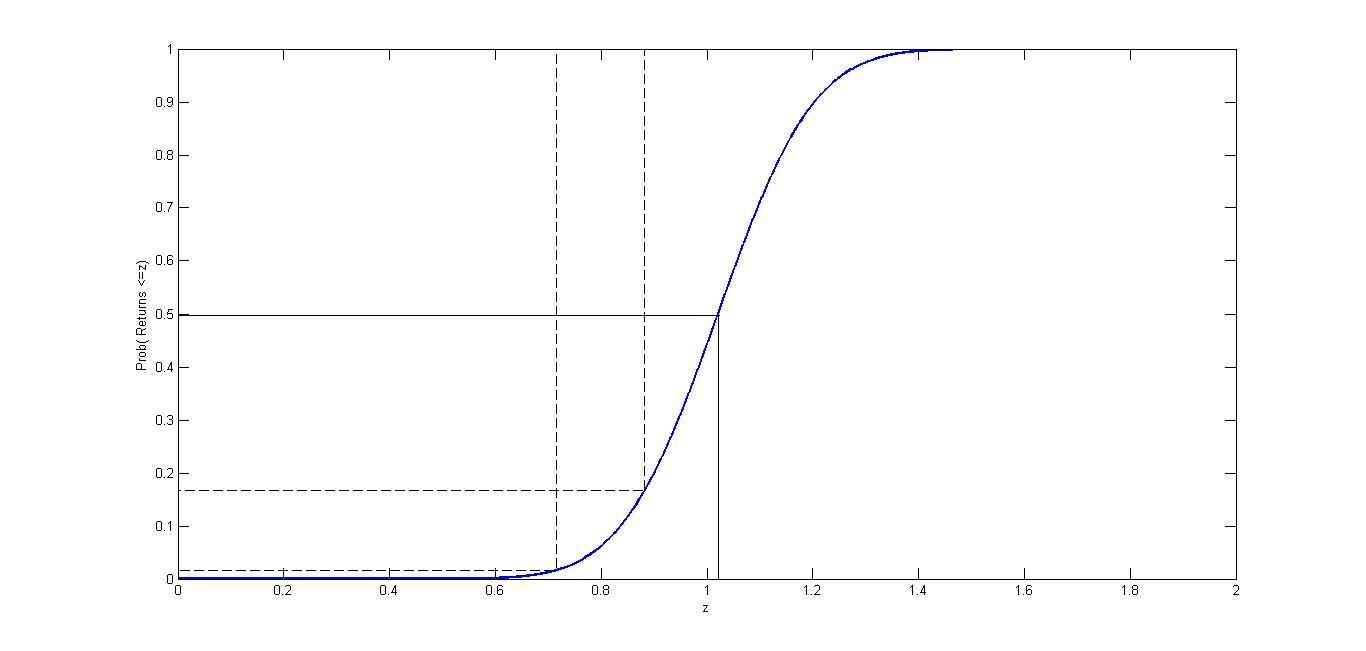
\includegraphics[width=6in]{kaavali.jpg}
\caption{Cumulative distributive function of returns for optimal portfolio}
\label{fig:1}
\end{figure}


Figure \ref{fig:1} plots the cumulative distribution of the return for the optimal portfolio. The
50\% probability level corresponds, on the horizontal axis, to the expected return. The loss
probability constraints are also drawn in the figure. Note that the 0.7 return (0.3 value at risk)
for a 97\% confidence level is the active constraint.



%Explain the intutive notion of higher returns stocks onlly
%operational and rest all selling
% Also high covariance related comments
%Most of the stocks are sold
% Bommalu 

\begin{thebibliography}{10}

\bibitem{1} Wikipedia
\bibitem{2} Portfolio optimization with linear and fixed transaction costs, .....
\end{thebibliography}






\end{document}